%%%%%%%%%%%%%%%%%%%%%%%%%%%%%%%%%%%%%%%%%%%%%%%%%%%%%%%%%%%%%%%%%%%%%%%%%%%%%%%%
%2345678901234567890123456789012345678901234567890123456789012345678901234567890
%        1         2         3         4         5         6         7         8

\documentclass[letterpaper, 10 pt, conference]{ieeeconf}  % Comment this line out
                                                          % if you need a4paper
%\documentclass[a4paper, 10pt, conference]{ieeeconf}      % Use this line for a4
                                                          % paper

\IEEEoverridecommandlockouts                              % This command is only
                                                          % needed if you want to
                                                          % use the \thanks command
\overrideIEEEmargins
% See the \addtolength command later in the file to balance the column lengths
% on the last page of the document



% The following packages can be found on http:\\www.ctan.org
\usepackage{graphics} % for pdf, bitmapped graphics files
\usepackage{epsfig} % for postscript graphics files
%\usepackage{subfigure} % ben: is this package allowed?
%\usepackage{mathptmx} % assumes new font selection scheme installed
%\usepackage{times} % assumes new font selection scheme installed
%\usepackage{amsmath} % assumes amsmath package installed
%\usepackage{amssymb}  % assumes amsmath package installed

\title{\LARGE \bf
On Physics-Based 3D Waypoint Generation for Autonomous Exploration in Mobile Robotics
}

%\author{ \parbox{3 in}{\centering Huibert Kwakernaak*
%         \thanks{*Use the $\backslash$thanks command to put information here}\\
%         Faculty of Electrical Engineering, Mathematics and Computer Science\\
%         University of Twente\\
%         7500 AE Enschede, The Netherlands\\
%         {\tt\small h.kwakernaak@autsubmit.com}}
%         \hspace*{ 0.5 in}
%         \parbox{3 in}{ \centering Pradeep Misra**
%         \thanks{**The footnote marks may be inserted manually}\\
%        Department of Electrical Engineering \\
%         Wright State University\\
%         Dayton, OH 45435, USA\\
%         {\tt\small pmisra@cs.wright.edu}}
%}

\author{Benjamin Adler and Jianwei Zhang% <-this % stops a space
\thanks{This work was not supported by any organization}% <-this % stops a space
\thanks{H. Kwakernaak is with Faculty of Electrical Engineering, Mathematics and Computer Science,
        University of Twente, 7500 AE Enschede, The Netherlands
        {\tt\small h.kwakernaak@autsubmit.com}}%
\thanks{P. Misra is with the Department of Electrical Engineering, Wright State University,
        Dayton, OH 45435, USA
        {\tt\small pmisra@cs.wright.edu}}%
}


\begin{document}



\maketitle
\thispagestyle{empty}
\pagestyle{empty}


%%%%%%%%%%%%%%%%%%%%%%%%%%%%%%%%%%%%%%%%%%%%%%%%%%%%%%%%%%%%%%%%%%%%%%%%%%%%%%%%

\begin{abstract}

This paper presents a novel, physics-based approach to generating waypoints, which are subsequently being used to steer a flying platform in three-dimensional space to map an outdoor environment. Because the algorithm relies on simple physical processes, it is both easy to understand and to implement in combination with traditional data structures. Generation of efficient sensor-trajectories for maximized information gain operates directly on unorganized point-clouds, creating a perfect fit for environment mapping with commonly user LIDAR sensors or time-of-flight cameras.

We also present the algorithm by simulating its performance in a virtual outdoor scenario.

\end{abstract}

%%%%%%%%%%%%%%%%%%%%%%%%%%%%%%%%%%%%%%%%%%%%%%%%%%%%%%%%%%%%%%%%%%%%%%%%%%%%%%%%


\section{Introduction}

Automatic model building has always been one of the most important parts of autonomous robotics. Exploration and mapping - as a subclass of this problem - has been the topic of many papers in recent years. The SLAM problem was first solved for two-dimensional mapping scenarios [thrun, freiburg etc.] and later-on expanded to three-dimensional environments [kinect-uav etc].

This paper presents a novel approach on increasing the efficiency of such mapping procedures. While the implementations of SLAM have improved greatly in recent years, one aspect of mapping three-dimensional environments was given comparatively little attention: finding the next best view. Typically, SLAM algorithms have been researched and developed on mobile platforms driving on flat surfaces. This setup does not require a high efficiency in exploration, as it does not inherently impose time constraints. The authors of this paper, however, are implementing exploration and mapping algorithms on a flying platform with a maximum flight time of about 15 minutes. Aiming to explore as much of the environment as possible within this limited time motivates an efficient way of finding sensor-poses (and in extension, -trajectories) that enable sensors to deliver as much information as quickly as possible.

\section{State of the Art}

Since the introduction of Thrun's SLAM approach, much work has been done to refine and extend the algorithm for use in both two- and threedimensional environments []. Finding the next best view, though, has never been a part of SLAM problem.

In general, frontier heuristic is popular, but how to do this in point cloud? low-res, physics spheres.


Occupancy grid maps are bound to 2d environments or voxel structures.

Multi-Level surface maps, Height maps don't allow for overhang.

e.g. ``Autonomous Exploration for 3D Map Learning'' by Johoo et al.

\section{Our approach}

Prior to the mapping process, the user creates a bounding volume as a representation of the region-of-interest around the vehicle's starting position, thereby defining the environment that is to be mapped. All generated viewpoints will be constrained to this volume, also ensuring that the UAV does not leave the given area. At initialization, a physics engine is set up with a detection volume at the bottom of the defined bounding volume. Whenever an object passes this area in physics computations, a ``calculate

\begin{figure*}[ht]
  \centering
    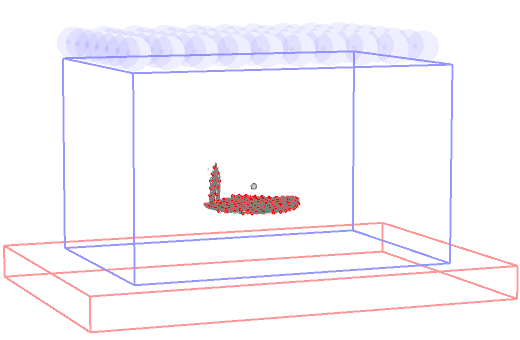
\includegraphics[width=0.23\textwidth]{images/expl1}
    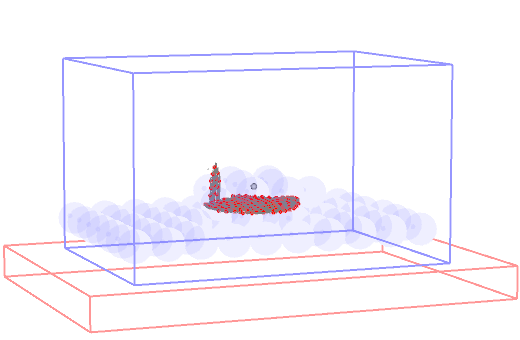
\includegraphics[width=0.23\textwidth]{images/expl2}
    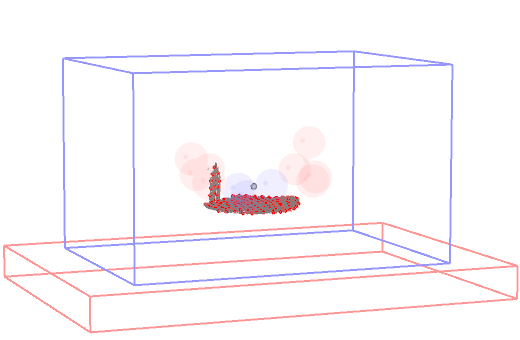
\includegraphics[width=0.23\textwidth]{images/expl3}
    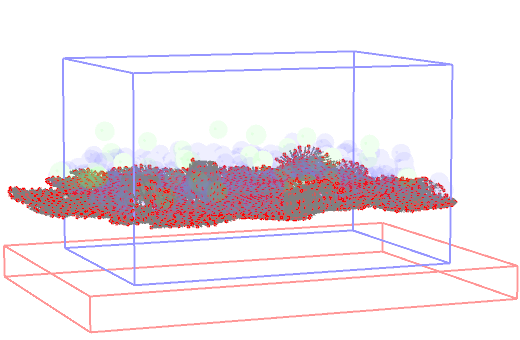
\includegraphics[width=0.23\textwidth]{images/process5}
    \caption{Mapping setup; bounding volume is blue, detection volume is red, vehicle position is grey, pointcloud for geometry reconstruction is grey and pointcloud for waypoint generation is red. Second figure shows sampling geometry interacting with pointcloud. Geometry hitting the red volume will be converted to a waypoint at the position it last hit a point from the pointcloud. The last figure shows generated pointcloud and leftover sampling geometry.}
    %\label{expl3}
\end{figure*}

As three-dimensional environment mapping is often implemented using laserscanners and time-of-flight cameras, unorganized point clouds are a very common type of sensor data. Finding the next best view in such a point cloud can be very hard, as the data itself does not supply any information about geometric structures such as corners, edges, surfaces and normals. Instead of trying to generate these details from the point cloud whenever it changes, our algorithm does not require such information.

The pointcloud itself is saved into two customized octrees which differ only in the allowed maximum density of points. One octree is used to capture all geometry for later surface reconstruction and thus allows for a very high density of points. The other octree is used for waypoint generation and only stores points if there are no other points whithin a distance of *dMin*, leading to comparatively little memory consumption. This density limitation is implemented by simple neighbor-queries common in most octree implementations.



Any sensor generating spatial occupancy information can be used, as the algorithm's input consists solely of geometry.

Spatially limited by defined exploration space, other input pre-existing sensor information and vehicle position.

Simulated annealing.

kugeln sind gut wgeen einfacher darstellung im speicher und, weil sie rutschen.

\subsection{3D Model / Data structures}

To operate on non-flat surfaces, we need appropriate data structures. Elevation maps don't work for no overhangs and multiple levels.

point cloud, octree

explain how. bullet, btghostobject

Bilder von fallenden Kugeln, abrutschen.

\subsection{Information Gain}

\begin{figure*}[ht]
  \centering
    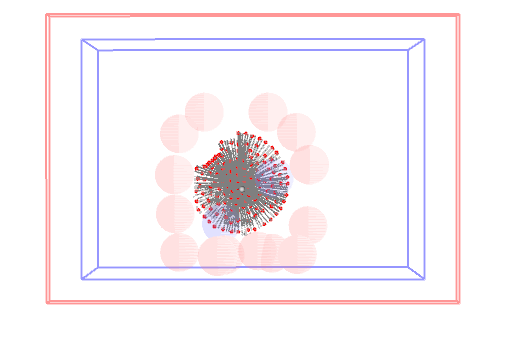
\includegraphics[width=0.2\textwidth]{images/process1}
    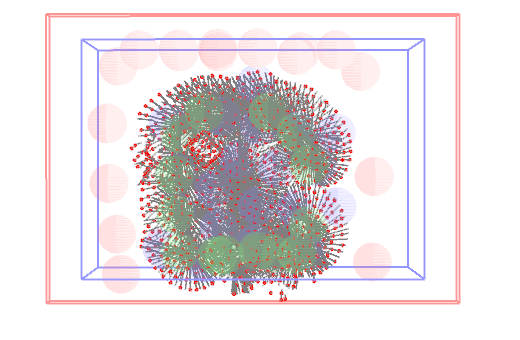
\includegraphics[width=0.2\textwidth]{images/process2}
    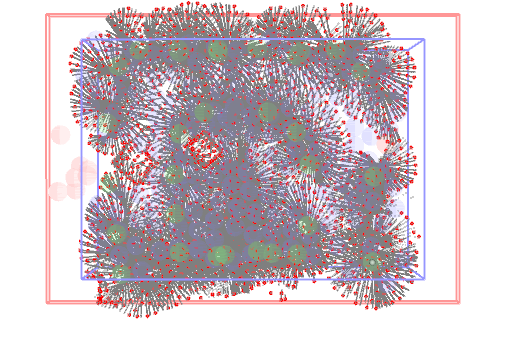
\includegraphics[width=0.2\textwidth]{images/process3}
    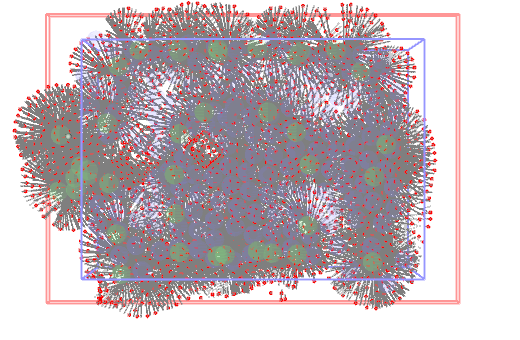
\includegraphics[width=0.2\textwidth]{images/process4}
    %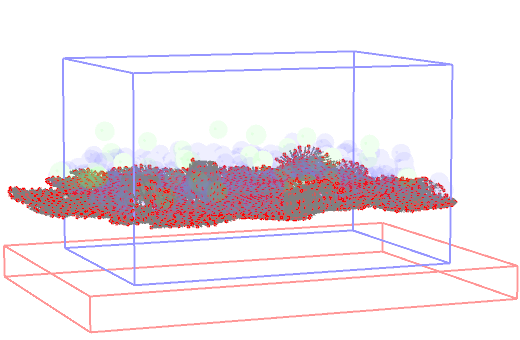
\includegraphics[width=0.2\textwidth]{images/process5}
    \caption{Multiple iterations of waypoint generation lead to a continuous scanning at the border between known and unknown environment.}
    %\label{expl3}
\end{figure*}

weil die kugeln, die von der kante fallen, (am meisten) zählen, bekomme ich immer wegpunkte mit dem größten information gain?!

\subsection{Computational complexity}

scalable resolution (sample sphere size / octree density)
simulated annealing length

\section{Experiments}
efficiency / performance
graph zeit vs number of points scanned
scalability durch Kugelgröße / Menge

\section{Outlook}

With the algorithm relying on collision detection between many static and dynamic objects, it is currently limited by the speed of collision detection. In general, physics-simulation in general and collision detection especially tends to lend itself well to parallelization using massively-parallel implementations on GPUs

more efficient with opencl -> from iterative to realtime
kugeln spucken in flugrichtung

collision avoidance! lass die kugeln liegen, fliege drüber, dann wird nichts passieren?!


%%%%%%%%%%%%%%%%%%%%%%%%%%%%%%%%%%%%%%%%%%%%%%%%%%%%%%%%%%%%%%%%%%%%%%%%%%%%%%%%
\section{ACKNOWLEDGMENTS}

The authors gratefully acknowledge the contribution of TAMS.


%%%%%%%%%%%%%%%%%%%%%%%%%%%%%%%%%%%%%%%%%%%%%%%%%%%%%%%%%%%%%%%%%%%%%%%%%%%%%%%%

References are important to the reader; therefore, each citation must be complete and correct. If at all possible, references should be commonly available publications.

\begin{thebibliography}{99}

\bibitem{c1}
J.G.F. Francis, The QR Transformation I, {\it Comput. J.}, vol. 4, 1961, pp 265-271.

\bibitem{c2}
H. Kwakernaak and R. Sivan, {\it Modern Signals and Systems}, Prentice Hall, Englewood Cliffs, NJ; 1991.

\bibitem{c3}
D. Boley and R. Maier, "A Parallel QR Algorithm for the Non-Symmetric Eigenvalue Algorithm", {\it in Third SIAM Conference on Applied Linear Algebra}, Madison, WI, 1988, pp. A20.

\end{thebibliography}

\end{document}

